\documentclass[12pt,letterpaper]{article}
\usepackage{graphicx,textcomp}
\usepackage{natbib}
\usepackage{setspace}
\usepackage{fullpage}
\usepackage{color}
\usepackage[reqno]{amsmath}
\usepackage{amsthm}
\usepackage{fancyvrb}
\usepackage{amssymb,enumerate}
\usepackage[all]{xy}
\usepackage{endnotes}
\usepackage{lscape}
\newtheorem{com}{Comment}
\usepackage{float}
\usepackage{hyperref}
\newtheorem{lem} {Lemma}
\newtheorem{prop}{Proposition}
\newtheorem{thm}{Theorem}
\newtheorem{defn}{Definition}
\newtheorem{cor}{Corollary}
\newtheorem{obs}{Observation}
\usepackage[compact]{titlesec}
\usepackage{dcolumn}
\usepackage{tikz}
\usetikzlibrary{arrows}
\usepackage{multirow}
\usepackage{xcolor}
\newcolumntype{.}{D{.}{.}{-1}}
\newcolumntype{d}[1]{D{.}{.}{#1}}
\definecolor{light-gray}{gray}{0.65}
\usepackage{url}
\usepackage{listings}
\usepackage{color}
\usepackage{verbatim} % includes comment blocks

\definecolor{codegreen}{rgb}{0,0.6,0}
\definecolor{codegray}{rgb}{0.5,0.5,0.5}
\definecolor{codepurple}{rgb}{0.58,0,0.82}
\definecolor{backcolour}{rgb}{0.95,0.95,0.92}

\lstdefinestyle{mystyle}{
	backgroundcolor=\color{backcolour},   
	commentstyle=\color{codegreen},
	keywordstyle=\color{magenta},
	numberstyle=\tiny\color{codegray},
	stringstyle=\color{codepurple},
	basicstyle=\footnotesize,
	breakatwhitespace=false,         
	breaklines=true,                 
	captionpos=b,                    
	keepspaces=true,                 
	numbers=left,                    
	numbersep=5pt,                  
	showspaces=false,                
	showstringspaces=false,
	showtabs=false,                  
	tabsize=2
}
\lstset{style=mystyle}
\newcommand{\Sref}[1]{Section~\ref{#1}}
\newtheorem{hyp}{Hypothesis}

\title{Problem Set 3}
\date{Due: November 20, 2021}
\author{Applied Stats/Quant Methods 1}


\begin{document}
	\maketitle
\begin{comment}
	\section*{Instructions}
	\begin{itemize}
		\item Please show your work! You may lose points by simply writing in the answer. If the problem requires you to execute commands in \texttt{R}, please include the code you used to get your answers. Please also include the \texttt{.R} file that contains your code. If you are not sure if work needs to be shown for a particular problem, please ask.
	\item Your homework should be submitted electronically on GitHub.
	\item This problem set is due before 23:59 on Sunday November 20, 2022. No late assignments will be accepted.
	\item Total available points for this homework is 80.
	\end{itemize}

\noindent In this problem set, you will run several regressions and create an add variable plot (see the lecture slides) in \texttt{R} using the \texttt{incumbents\_subset.csv} dataset. Include all of your code.

		\vspace{.25cm}
	\end{comment}

  \section*{Data} 
  \lstinputlisting[language=R, firstline=61, lastline=61]{PS03.R}
	%\vspace{.5cm}

\section*{Question 1}
%\vspace{.25cm}
\noindent We are interested in knowing how the difference in campaign spending between incumbent and challenger affects the incumbent's vote share. 
	\begin{enumerate}
		\item Run a regression where the outcome variable is \texttt{voteshare} and the explanatory variable is \texttt{difflog}.	
		  The function call to generate the model is:
	\lstinputlisting[language=R, firstline=100, lastline=100]{PS03.R}
	The results are: 
    
% Table created by stargazer v.5.2.3 by Marek Hlavac, Social Policy Institute. E-mail: marek.hlavac at gmail.com
% Date and time: Mon, Nov 14, 2022 - 16:58:02
\begin{table}[!htbp] \centering 
  \caption{Vote share as a function of Differental Spending} 
  \label{tab:vote_spend} 
\begin{tabular}{@{\extracolsep{5pt}}lc} 
\\[-1.8ex]\hline 
\hline \\[-1.8ex] 
 & \multicolumn{1}{c}{\textit{Dependent variable:}} \\ 
\cline{2-2} 
\\[-1.8ex] & voteshare \\ 
\hline \\[-1.8ex] 
 difflog & 0.041666$^{***}$ \\ 
  & (0.000968) \\ 
  & \\ 
 Constant & 0.579031$^{***}$ \\ 
  & (0.002251) \\ 
  & \\ 
\hline \\[-1.8ex] 
Observations & 3,193 \\ 
R$^{2}$ & 0.367341 \\ 
Adjusted R$^{2}$ & 0.367143 \\ 
Residual Std. Error & 0.078673 (df = 3191) \\ 
F Statistic & 1,852.791000$^{***}$ (df = 1; 3191) \\ 
\hline 
\hline \\[-1.8ex] 
\textit{Note:}  & \multicolumn{1}{r}{$^{*}$p$<$0.1; $^{**}$p$<$0.05; $^{***}$p$<$0.01} \\ 
\end{tabular} 
\end{table}  

		\item Make a scatterplot of the two variables and add the regression line. 	
	\begin{figure}
		  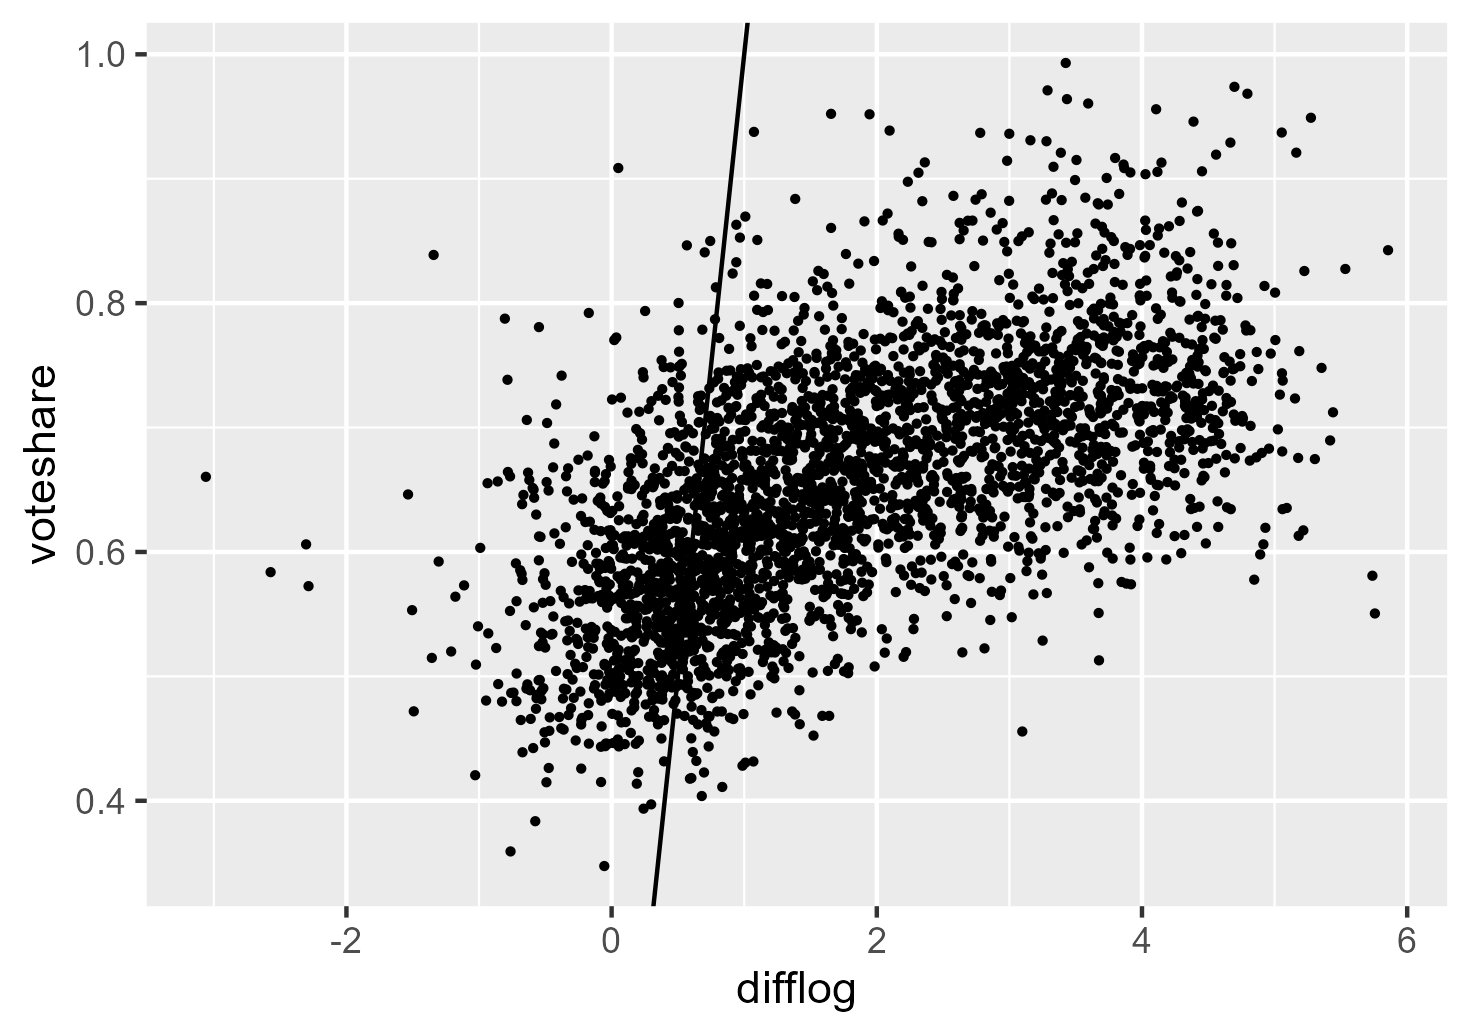
\includegraphics[width=0.9\textwidth]{Graphics/vote_spend.png}
		  \caption{Vote share as a function of Differental Spending}
		  \label{fig:vote_spend}
	\end{figure}
		
		\item Save the residuals of the model in a separate object.	

	\lstinputlisting[language=R, firstline=109, lastline=109]{PS03.R}

		\item Write the prediction equation.
		
    \textbf{Prediction Equation} 
    $voteshare = 0.579031 + (0.041666) * difflog$
    ie the voteshare is 0.579031 when difflog is 0
    it increases by 0.041666 for each unit increase in difflog

	\end{enumerate}

\newpage

\section*{Question 2}
\noindent We are interested in knowing how the difference between incumbent and challenger's spending and the vote share of the presidential candidate of the incumbent's party are related.\vspace{.25cm}

	\begin{enumerate}
		\item Run a regression where the outcome variable is \texttt{presvote} and the explanatory variable is \texttt{difflog}.	
		
  The function call to generate the model is:
	\lstinputlisting[language=R, firstline=155, lastline=155]{PS03.R}
  The results are in table~\ref{tab:pres_spend}
  
% Table created by stargazer v.5.2.3 by Marek Hlavac, Social Policy Institute. E-mail: marek.hlavac at gmail.com
% Date and time: Mon, Nov 14, 2022 - 16:58:04
\begin{table}[!htbp] \centering 
  \caption{Presidential vote share as a function of Differental Spending} 
  \label{tab:pres_spend} 
\begin{tabular}{@{\extracolsep{5pt}}lc} 
\\[-1.8ex]\hline 
\hline \\[-1.8ex] 
 & \multicolumn{1}{c}{\textit{Dependent variable:}} \\ 
\cline{2-2} 
\\[-1.8ex] & presvote \\ 
\hline \\[-1.8ex] 
 difflog & 0.023837$^{***}$ \\ 
  & (0.001359) \\ 
  & \\ 
 Constant & 0.507583$^{***}$ \\ 
  & (0.003161) \\ 
  & \\ 
\hline \\[-1.8ex] 
Observations & 3,193 \\ 
R$^{2}$ & 0.087951 \\ 
Adjusted R$^{2}$ & 0.087665 \\ 
Residual Std. Error & 0.110442 (df = 3191) \\ 
F Statistic & 307.715400$^{***}$ (df = 1; 3191) \\ 
\hline 
\hline \\[-1.8ex] 
\textit{Note:}  & \multicolumn{1}{r}{$^{*}$p$<$0.1; $^{**}$p$<$0.05; $^{***}$p$<$0.01} \\ 
\end{tabular} 
\end{table}  

		
		\item Make a scatterplot of the two variables and add the regression line.
	\begin{figure}
		  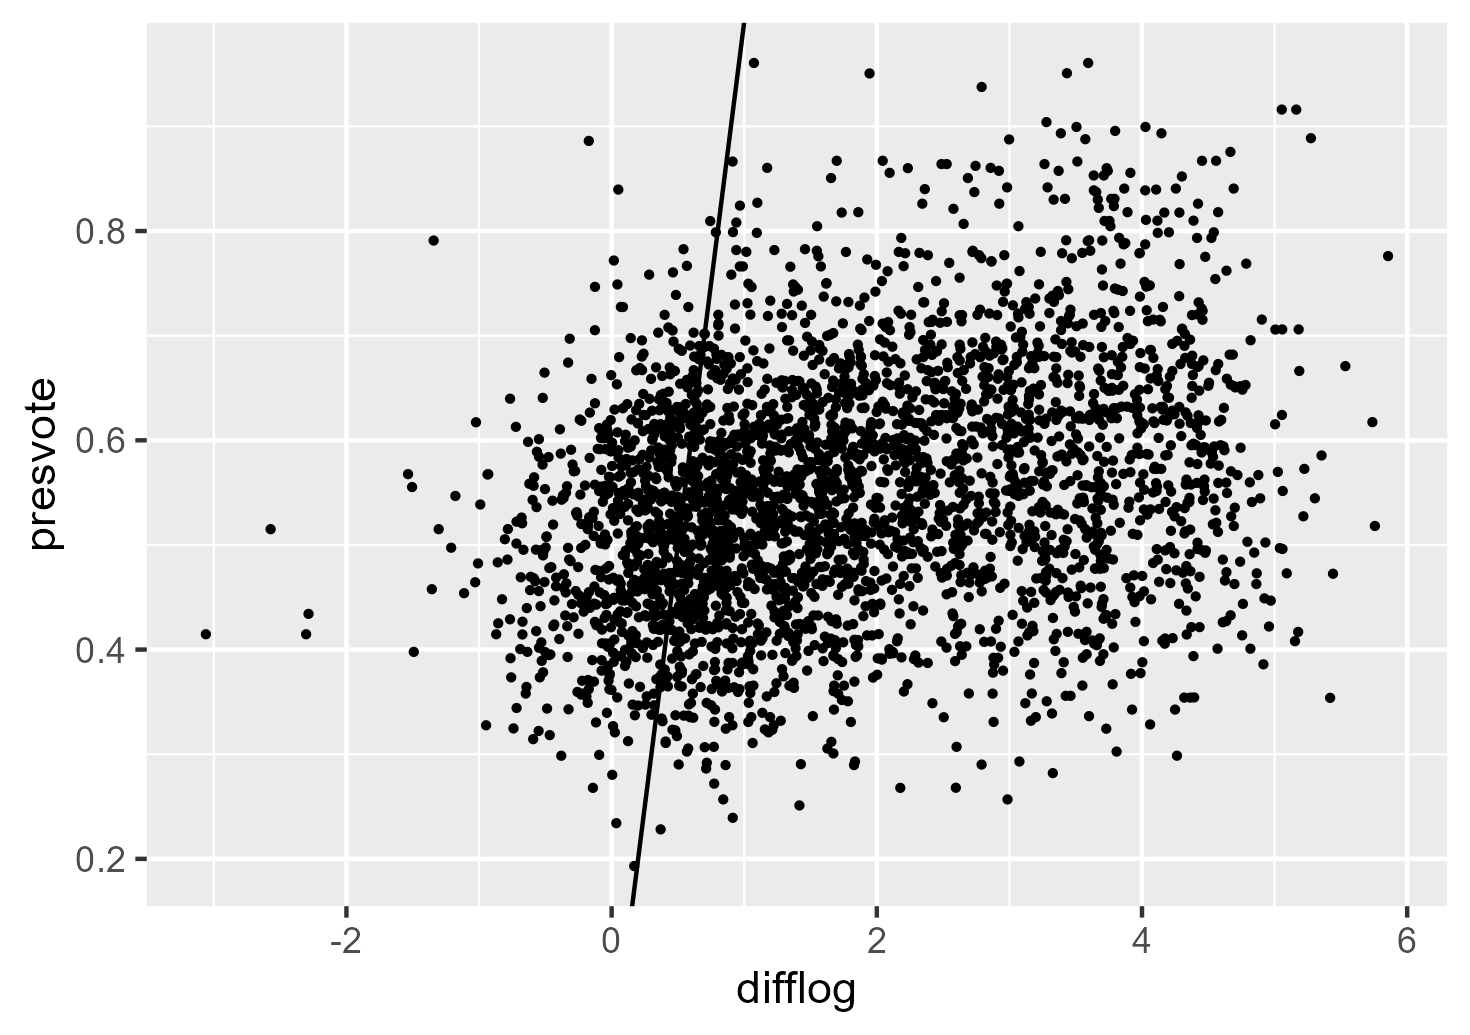
\includegraphics[width=0.9\textwidth]{Graphics/pres_spend.png}
		  \caption{Presidential vote share as a function of Differental Spending}
		  \label{fig:pres_spend}
	\end{figure}
		
		\item Save the residuals of the model in a separate object.	
	\lstinputlisting[language=R, firstline=164, lastline=164]{PS03.R}
		
		\item Write the prediction equation.
    \textbf{Prediction Equation} 
     $presvote = 0.507583 + (0.023837) * difflog$
     ie the presvote is 0.507583 when difflog is 0
        it increases by 0.023837 for each unit increase in difflog

	\end{enumerate}

	\newpage	

\section*{Question 3}

\noindent We are interested in knowing how the vote share of the presidential candidate of the incumbent's party is associated with the incumbent's electoral success.
	\vspace{.25cm}
	\begin{enumerate}
		\item Run a regression where the outcome variable is \texttt{voteshare} and the explanatory variable is \texttt{presvote}.
    The function call to generate the model is:
  	\lstinputlisting[language=R, firstline=155, lastline=155]{PS03.R}
    and the results are in~\ref{tab:vote_pres}
    
% Table created by stargazer v.5.2.3 by Marek Hlavac, Social Policy Institute. E-mail: marek.hlavac at gmail.com
% Date and time: Mon, Nov 14, 2022 - 16:58:05
\begin{table}[!htbp] \centering 
  \caption{Vote share as a function of Presidential vote share} 
  \label{tab:vote_pres} 
\begin{tabular}{@{\extracolsep{5pt}}lc} 
\\[-1.8ex]\hline 
\hline \\[-1.8ex] 
 & \multicolumn{1}{c}{\textit{Dependent variable:}} \\ 
\cline{2-2} 
\\[-1.8ex] & voteshare \\ 
\hline \\[-1.8ex] 
 presvote & 0.388018$^{***}$ \\ 
  & (0.013493) \\ 
  & \\ 
 Constant & 0.441330$^{***}$ \\ 
  & (0.007599) \\ 
  & \\ 
\hline \\[-1.8ex] 
Observations & 3,193 \\ 
R$^{2}$ & 0.205814 \\ 
Adjusted R$^{2}$ & 0.205565 \\ 
Residual Std. Error & 0.088146 (df = 3191) \\ 
F Statistic & 826.950200$^{***}$ (df = 1; 3191) \\ 
\hline 
\hline \\[-1.8ex] 
\textit{Note:}  & \multicolumn{1}{r}{$^{*}$p$<$0.1; $^{**}$p$<$0.05; $^{***}$p$<$0.01} \\ 
\end{tabular} 
\end{table}  


		\item Make a scatterplot of the two variables and add the regression line. 
	\begin{figure}
		  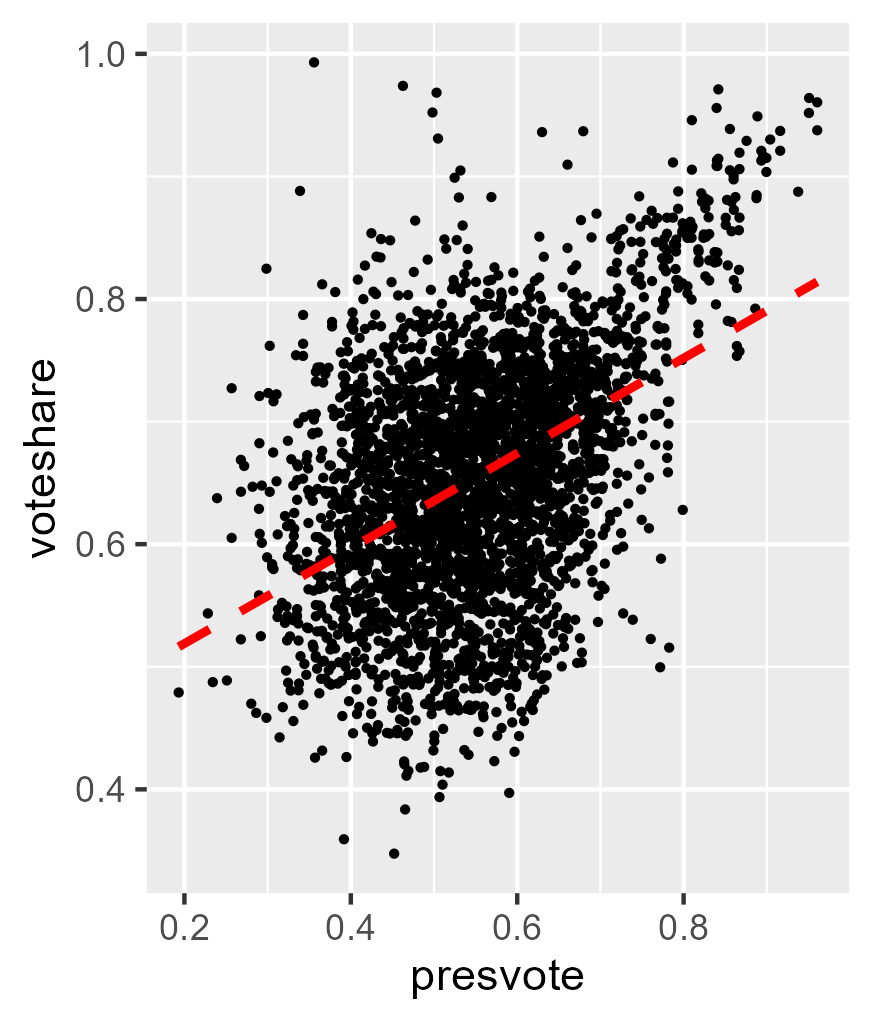
\includegraphics[width=0.9\textwidth]{Graphics/vote_pres.png}
		  \caption{Vote share as a function of Presidential vote share}
		  \label{fig:vote_pres}
	\end{figure}

		\item Write the prediction equation.
		
    \textbf{Prediction Equation} 

     $voteshare = 0.441330 + (0.388018) * presvote$
     ie the voteshare is 0.441330 when presvote is 0
        it increases by 0.388018 for each unit increase in presvote
	\end{enumerate}
	
\newpage	

\section*{Question 4}
\noindent The residuals from part (a) tell us how much of the variation in \texttt{voteshare} is $not$ explained by the difference in spending between incumbent and challenger. The residuals in part (b) tell us how much of the variation in \texttt{presvote} is $not$ explained by the difference in spending between incumbent and challenger in the district.
	\begin{enumerate}
		\item Run a regression where the outcome variable is the residuals from Question 1 and the explanatory variable is the residuals from Question 2.	
		
  The function call to generate the model is:
	\lstinputlisting[language=R, firstline=209, lastline=209]{PS03.R}

	The results of the linear model are:
  
% Table created by stargazer v.5.2.3 by Marek Hlavac, Social Policy Institute. E-mail: marek.hlavac at gmail.com
% Date and time: Thu, Nov 17, 2022 - 13:43:55
\begin{table}[!htbp] \centering 
  \caption{Incumbent's vote share residuals as a function of Presidential vote share residuals} 
  \label{tab:residuals} 
\begin{tabular}{@{\extracolsep{5pt}}lc} 
\\[-1.8ex]\hline 
\hline \\[-1.8ex] 
 & \multicolumn{1}{c}{\textit{Dependent variable:}} \\ 
\cline{2-2} 
\\[-1.8ex] & resid\_vote\_spend \\ 
\hline \\[-1.8ex] 
 resid\_pres\_spend & 0.256877$^{***}$ \\ 
  & (0.011762) \\ 
  & \\ 
 Constant & $-$0.000000 \\ 
  & (0.001299) \\ 
  & \\ 
\hline \\[-1.8ex] 
Observations & 3,193 \\ 
R$^{2}$ & 0.130038 \\ 
Adjusted R$^{2}$ & 0.129765 \\ 
Residual Std. Error & 0.073380 (df = 3191) \\ 
F Statistic & 476.974700$^{***}$ (df = 1; 3191) \\ 
\hline 
\hline \\[-1.8ex] 
\textit{Note:}  & \multicolumn{1}{r}{$^{*}$p$<$0.1; $^{**}$p$<$0.05; $^{***}$p$<$0.01} \\ 
\end{tabular} 
\end{table}  


		\item Make a scatterplot of the two residuals and add the regression line.
	\begin{figure}
		  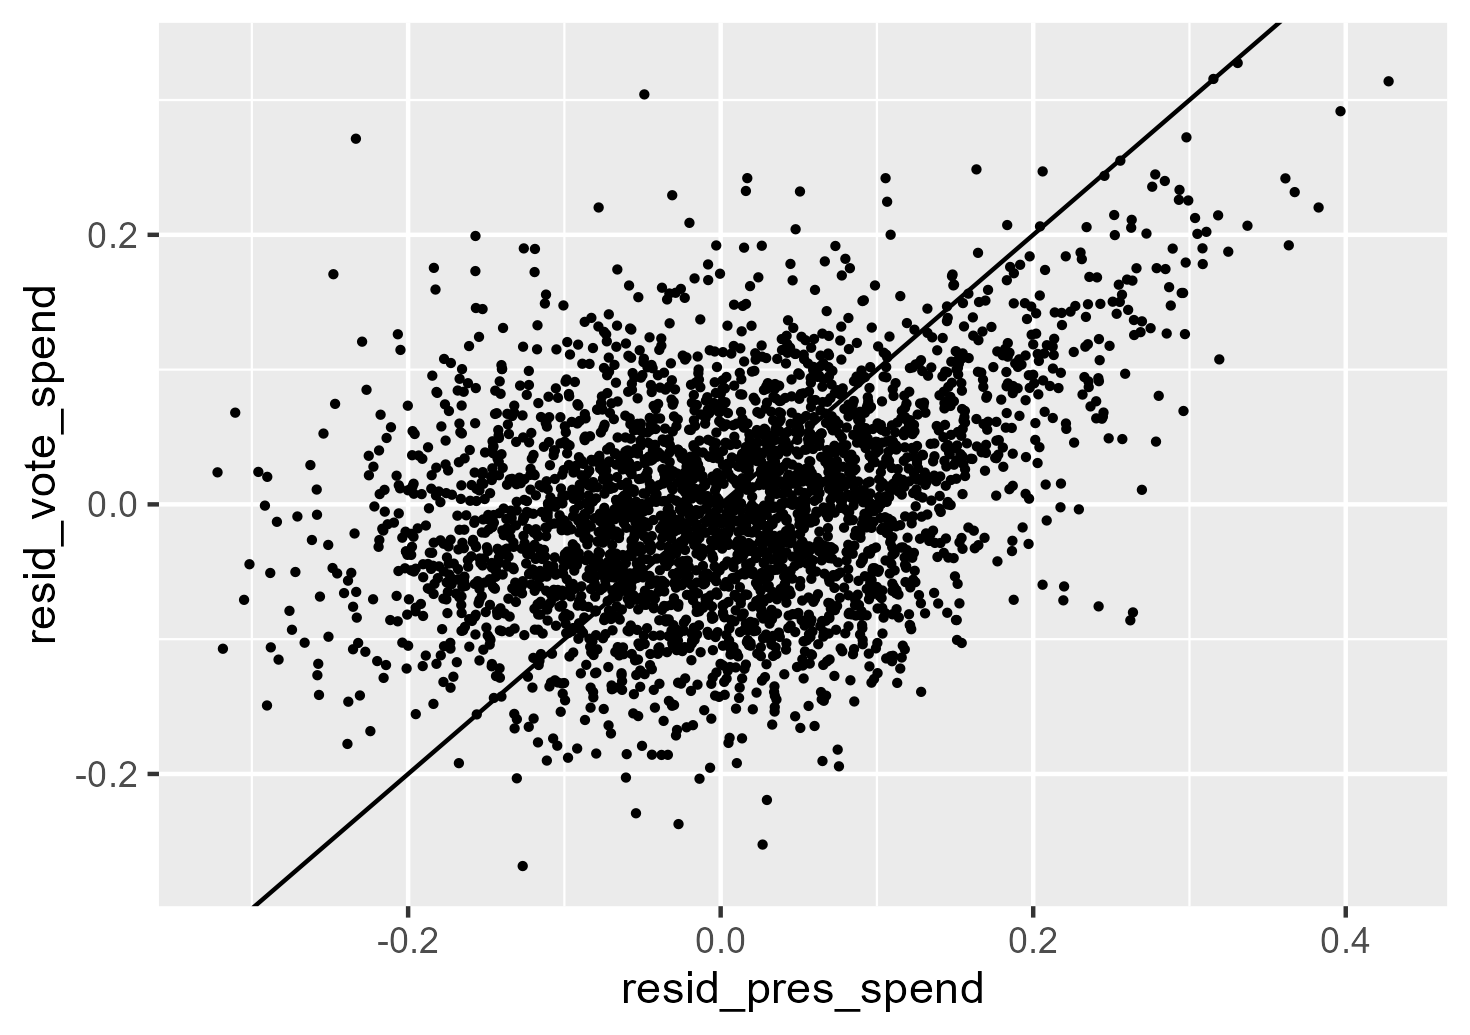
\includegraphics[width=0.9\textwidth]{Graphics/residuals.png}
		  \caption{Vote share residuals as a function of Presidential vote share residuals}
		  \label{fig:residuals}
	\end{figure}

		\item Write the prediction equation.
		
	\textbf{Prediction Equation}
	voteshare residuals  = -5.207e-18 + (0.2569) * presvote residuals
	ie the voteshare residual value is -5.207e-18 when presvote residual value is 0
	   it increases by 0.2569 for each unit increase in presvote residuals

  ie the value of the incumbent vote share not accounted for by the difference in incumbent spending increases by 0.2569 for each unit increase in the value of the unidentified factors which cause an increase in presidential vote share.

	\end{enumerate}
	
	\newpage	

\section*{Question 5}
\noindent What if the incumbent's vote share is affected by both the president's popularity and the difference in spending between incumbent and challenger? 
	\begin{enumerate}
		\item Run a regression where the outcome variable is the incumbent's \texttt{voteshare} and the explanatory variables are \texttt{difflog} and \texttt{presvote}.	
		
  The function call to generate the model is:
	\lstinputlisting[language=R, firstline=320, lastline=320]{PS03.R}

	The results of the linear model are:
  
% Table created by stargazer v.5.2.3 by Marek Hlavac, Social Policy Institute. E-mail: marek.hlavac at gmail.com
% Date and time: Thu, Nov 17, 2022 - 14:31:11
\begin{table}[!htbp] \centering 
  \caption{Vote share as a function of Presidential vote share and differential spending} 
  \label{tab:vote_spend_pres} 
\begin{tabular}{@{\extracolsep{5pt}}lcc} 
\\[-1.8ex]\hline 
\hline \\[-1.8ex] 
 & \multicolumn{2}{c}{\textit{Dependent variable:}} \\ 
\cline{2-3} 
\\[-1.8ex] & voteshare & resid\_vote\_spend \\ 
\\[-1.8ex] & (1) & (2)\\ 
\hline \\[-1.8ex] 
 presvote & 0.256877$^{***}$ &  \\ 
  & (0.011764) &  \\ 
  & & \\ 
 difflog & 0.035543$^{***}$ &  \\ 
  & (0.000946) &  \\ 
  & & \\ 
 resid\_pres\_spend &  & 0.256877$^{***}$ \\ 
  &  & (0.011762) \\ 
  & & \\ 
 Constant & 0.448644$^{***}$ & $-$0.000000 \\ 
  & (0.006330) & (0.001299) \\ 
  & & \\ 
\hline \\[-1.8ex] 
Observations & 3,193 & 3,193 \\ 
R$^{2}$ & 0.449610 & 0.130038 \\ 
Adjusted R$^{2}$ & 0.449265 & 0.129765 \\ 
Residual Std. Error & 0.073391 (df = 3190) & 0.073380 (df = 3191) \\ 
F Statistic & 1,302.947000$^{***}$ (df = 2; 3190) & 476.974700$^{***}$ (df = 1; 3191) \\ 
\hline 
\hline \\[-1.8ex] 
\textit{Note:}  & \multicolumn{2}{r}{$^{*}$p$<$0.1; $^{**}$p$<$0.05; $^{***}$p$<$0.01} \\ 
\end{tabular} 
\end{table}  


  The additional variables are plotted in~\ref{fig:add_var}.
	\begin{figure}
		  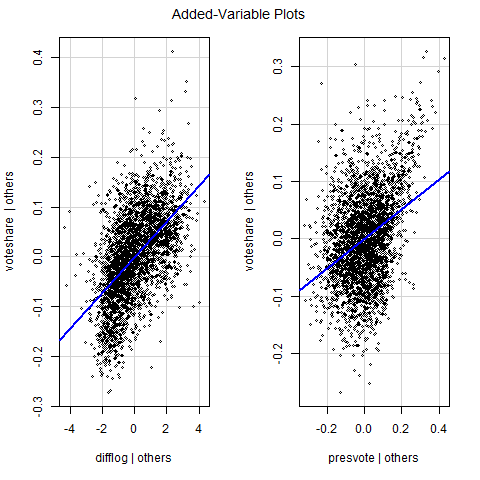
\includegraphics[width=1.0\textwidth]{Graphics/add_variable.png}
		  \caption{Vote share as a function of differential spending and presidential vote share}
		  \label{fig:add_var}
	\end{figure}


		\item Write the prediction equation.	\vspace{5cm}

  \textbf{Prediction Equation }
   $voteshare = 0.4486442 + (0.0355431) * difflog + (0.2568770) * presvote$

  ie the voteshare is 0.4486442 when difflog and presvote are 0
    it increases by 0.0355431 for each unit increase in difflog
           (holding presvote constant)
    it increases by 0.2568770 for each unit increase in presvote
           (holding difflog constant)

		\item What is it in this output that is identical to the output in Question 4? Why do you think this is the case?
    
    The coefficient for residual president share as a function of incumbent spending (Q4) is the same as the coefficient for presidential vote share.(0.256877)

    In model 5, the coefficient for presvote is a partial predictor, with difflog held constant.  In model 2, the residuals represent the variation in the value of the presidential vote, excluding difflog (which was specifically included as a predictor).  In both models, we are getting a predictive value for presvote on voteshare, with difflog excluded/controlled.

	\end{enumerate}


\newpage

\appendix{Appendix - Code}
	\lstinputlisting[language=R]{PS03.R}  

\end{document}
